\documentclass[11pt,colorlinks=true]{article}
\usepackage[margin=3cm]{geometry}



\usepackage[utf8x]{inputenc}
\usepackage[english,russian]{babel}
\usepackage{cmap}

\usepackage{amsmath}
\usepackage{amsthm}
\usepackage{bm}
\usepackage{bbold}
\usepackage{amssymb}

\usepackage{graphicx}


\usepackage{hyperref}


\DeclareMathOperator{\T}{T}
\DeclareMathOperator{\tr}{tr}
\DeclareMathOperator{\Tr}{Tr} 
\DeclareMathOperator{\MSE}{MSE} 
\DeclareMathOperator{\E}{E}
\DeclareMathOperator{\D}{D}

\newtheorem{theorem}{Теорема}
\newtheorem{lemma}{Лемма}
\newtheorem{corollary}{Следствие}
\newtheorem{statement}{Утверждение}
\newtheorem{note}{Замечание}
\newtheorem{theorem+}{Теорема Гаусса-Маркова}
\newtheorem{proposition}{Предложение}

\begin{document}

	\thispagestyle{empty}
%
	\begin{center}
		Санкт-Петербургский государственный университет \\
		\vspace{0.3cm}	
		Прикладная математика и информатика \\
		\vspace{0.3cm}
		Кафедра статистического моделирования \\
		
		\vspace{6cm}			   	
			
			\vspace{0.3cm}	
			%\vspace{2cm}	
			 {\huge Нейронные сети для изображений} \\
			 \vspace{0.5cm}
									Петраков Михаил \\
			Лунев Иван \\
			

			\vspace{10cm}	

		Санкт-Петербург \\
				2019
	\end{center}
	
\newpage


\tableofcontents

\newpage

\section{Введение}
Наилучшие результаты в области распознавания изображений показала Convolutional Neural Network или сверточная нейронная сеть (далее – СНС). Успех обусловлен возможностью учета двумерной топологии изображения, в отличие от многослойного персептрона. 

Сверточные нейронные сети представляют собой измененную разновидность многослойных персептронов (MLP). Нейроны в СНС имеют общий вес в отличие от MLP, где каждый нейрон имеет отдельный вектор весов. Такое распределение весов в конечном итоге приводит к уменьшению общего количества обучаемых весов, что приводит к разреженности. Используя стратегию распределения весов, нейроны могут выполнять свертки данных с помощью ядра свертки. Затем следует операция объединения, которая как форма нелинейной понижающей дискретизации постепенно уменьшает пространственный размер представления, тем самым уменьшая объем вычислений и параметров в сети.

Сверточные нейронные сети обеспечивают частичную устойчивость к изменениям масштаба, смещениям, поворотам, смене ракурса и прочим искажениям. Сверточные нейронные сети объединяют три архитектурных идеи, для обеспечения инвариантности к изменению масштаба, повороту сдвигу и пространственным искажениям:
\begin{itemize}
	\item локальные рецепторные поля (обеспечивают локальную двумерную связность нейронов);
	\item общие синаптические коэффициенты (обеспечивают детектирование некоторых черт в любом месте изображения и уменьшают общее число весовых коэффициентов);
	\item иерархическая организация с пространственными подвыборками.
\end{itemize}

\section{Структура СНС}
СНС состоит из разных видов слоев: сверточные (convolutional) слои, субдискретизирующие (subsampling, подвыборка) слои и слои «обычной» нейронной сети – персептрона, в соответствии с рисунком.

\begin{figure}[h]
		\begin{center}
				\begin{minipage}[h]{1\linewidth}
					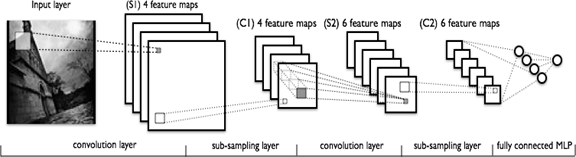
\includegraphics[width=1\linewidth]{structure}
				\end{minipage}
			\end{center}
		\end{figure}
	
Первые два типа слоев (convolutional, subsampling), чередуясь между собой, формируют входной вектор признаков для многослойного персептрона.

Свое название сверточная сеть получила по названию операции – свертка, суть которой будет описана дальше. 

Основной причиной успеха СНС стало концепция общих весов. Несмотря на большой размер, эти сети имеют небольшое количество настраиваемых параметров. СНС могут быстро работать на последовательной машине и быстро обучаться за счет чистого распараллеливания процесса свертки по каждой карте, а также обратной свертки при распространении ошибки по сети.

\subsection{Входной слой}

Так как рассматриваем применение СНС для изображений, то в качестве входных данных рассматриваем  изображения nхm пикселей.

Входной слой учитывает двумерную топологию изображений и состоит из нескольких карт (матриц), карта может быть одна, в том случае, если изображение представлено в оттенках серого, иначе их 3, где каждая карта соответствует изображению с конкретным каналом (красным, синим и зеленым).

\subsection{Сверточный слой}

Сверточный слой представляет из себя набор карт, у каждой карты есть синаптическое ядро (в разных источниках его называют по-разному: сканирующее ядро или фильтр). 

Количество карт определяется требованиями к задаче, если взять большое количество карт, то повысится качество распознавания, но увеличится вычислительная сложность. Исходя из анализа научных статей, в большинстве случаев предлагается брать соотношение один к двум, то есть каждая карта предыдущего слоя (например, у первого сверточного слоя, предыдущим является входной) связана с двумя картами сверточного слоя.

Ядро представляет из себя фильтр или окно, которое скользит по всей области предыдущей карты и находит определенные признаки объектов. Например, если сеть обучали на множестве лиц, то одно из ядер могло бы в процессе обучения выдавать наибольший сигнал в области глаза, рта, брови или носа, другое ядро могло бы выявлять другие признаки. Размер ядра обычно берут в пределах от 3х3 до 7х7. Если размер ядра маленький, то оно не сможет выделить какие-либо признаки, если слишком большое, то увеличивается количество связей между нейронами. Также размер ядра выбирается таким, чтобы размер карт сверточного слоя был четным, это позволяет не терять информацию при уменьшении размерности в объединяющем слое, описанном ниже. 

Ядро представляет собой систему разделяемых весов или синапсов, это одна из главных особенностей сверточной нейросети. В обычной многослойной сети очень много связей между нейронами, то есть синапсов, что весьма замедляет процесс детектирования. В сверточной сети – наоборот, общие веса позволяет сократить число связей и позволить находить один и тот же признак по всей области изображения.

Изначально значения каждой карты сверточного слоя равны 0. Значения весов ядер задаются случайным образом в области от -0.5 до 0.5. Ядро скользит по предыдущей карте и производит операцию свертка, которая часто используется для обработки изображений, формула:
\begin{equation*}
(\mathsf{x} * \mathsf{w})[\mathsf{i},\mathsf{j}] = \sum \limits_{\mathsf{a}} \sum \limits_{\mathsf{b}} \mathsf{w}_{\mathsf{ab}} \mathsf{x}[\mathsf{i} + \mathsf{a}, \mathsf{j} + \mathsf{b}]
\end{equation*}

$\mathsf{x}[i,j]$ - исходные признаки, пиксели $n \times m$ изображения; 

$\mathsf{w}_{ab}$ - ядро свертки, где считаем, что ядро является прямоугольным, а a и b длины его сторон. В случае, когда изображение цветное, для ядра добавляется <<глубина>>, равная~3.

Неформально эту операцию можно описать следующим образом — окном проходим с заданным шагом (обычно 1) все изображение, на каждом шаге поэлементно умножаем содержимое окна на ядро, результат суммируется и записывается в матрицу результата:

\begin{figure}[h]
	\begin{center}
		\begin{minipage}[h]{1\linewidth}
			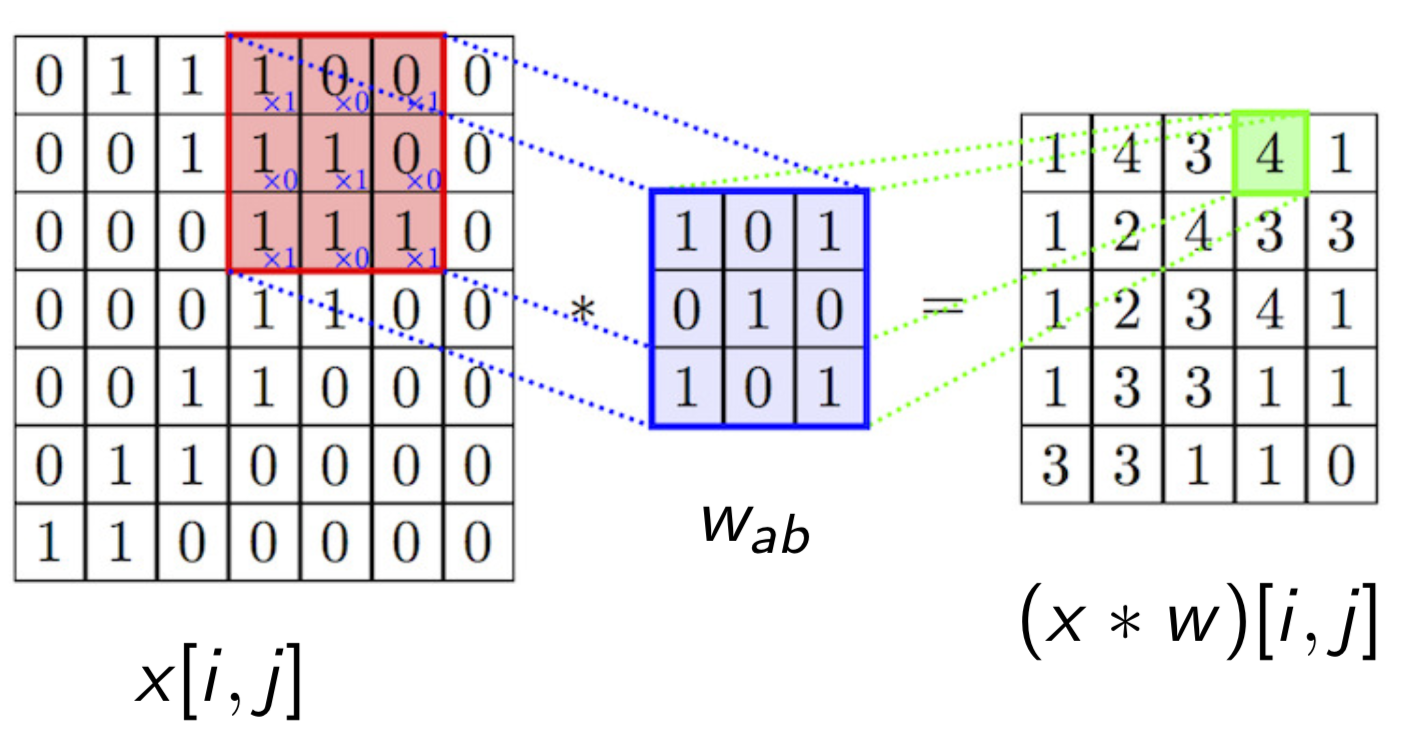
\includegraphics[width=0.8\linewidth]{sv}
		\end{minipage}
	\end{center}
\end{figure}

При этом в зависимости от метода обработки краев исходной матрицы результат может быть меньше исходного изображения (valid), такого же размера (same) или большего размера (full), в соответствии с рисунком:

\begin{figure}[h]
	\begin{center}
		\begin{minipage}[h]{1\linewidth}
			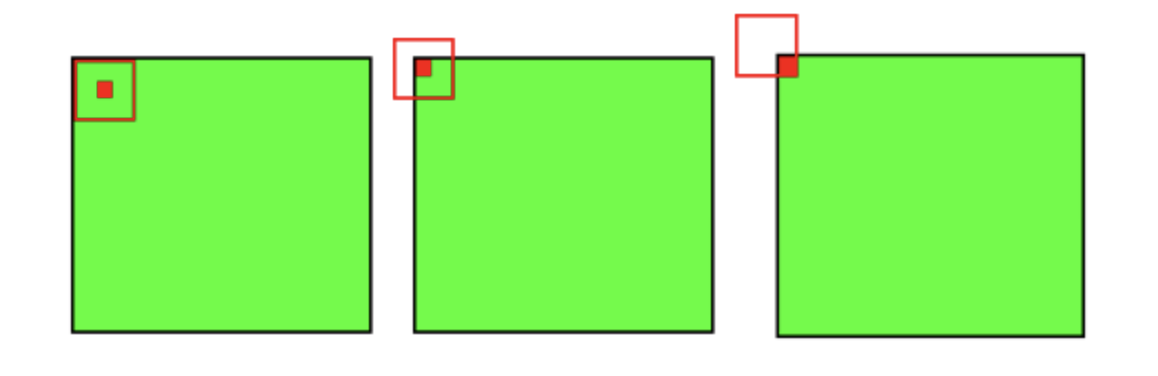
\includegraphics[width=0.6\linewidth]{zero_pad}
		\end{minipage}
	\end{center}
\end{figure}

В упрощенном виде этот слой можно описать формулой: 
\begin{figure}[h]
	\begin{center}
		\begin{minipage}[h]{1\linewidth}
			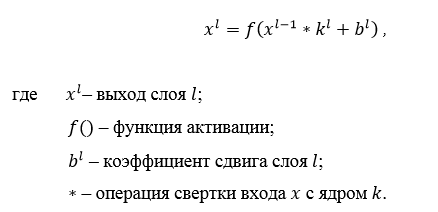
\includegraphics[width=0.6\linewidth]{conv_l}
		\end{minipage}
	\end{center}
\end{figure}



\newpage
\subsection{Объединяющий слой}

Подвыборочный слой также, как и сверточный имеет карты, но их количество совпадает с предыдущим (сверточным) слоем. Цель слоя – уменьшение размерности карт предыдущего слоя. Если на предыдущей операции свертки уже были выявлены некоторые признаки, то для дальнейшей обработки настолько подробное изображение уже не нужно, и оно уплотняется до менее подробного. К тому же фильтрация уже ненужных деталей помогает не переобучаться. 
В процессе сканирования ядром объединяющего слоя карты предыдущего слоя, сканирующее ядро, не пересекается в отличие от сверточного слоя. 

 Объединяющий слой нейронов -- это необучаемая свёртка с щагом $\mathsf{h} >1$, агрегирующая данные прямоугольной области $\mathsf{h} \times \mathsf{h}$:

    \begin{center}
    	$\mathsf{y}[\mathsf{i},\mathsf{j}] = \mathsf{F}(\mathsf{x}[\mathsf{hi},\mathsf{hj}],\dots,\mathsf{x}[\mathsf{hi} + \mathsf{h} - 1, \mathsf{hj} + \mathsf{h} - 1])$,
    \end{center}
гду $\mathsf{F}$ -- агрегирующая функция: max, average и т.п.

\begin{figure}[h]
	\begin{center}
		\begin{minipage}[h]{1\linewidth}
			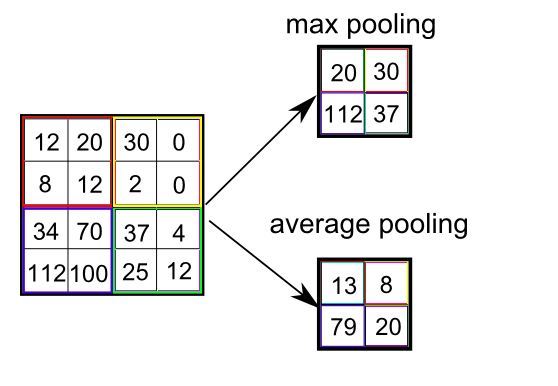
\includegraphics[width=0.7\linewidth]{mp}
		\end{minipage}
	\end{center}
\end{figure}

Формально данный слой, с добавление функции активации (обычно RelU), может быть описан формулой: 

\begin{figure}[h]
	\begin{center}
		\begin{minipage}[h]{1\linewidth}
			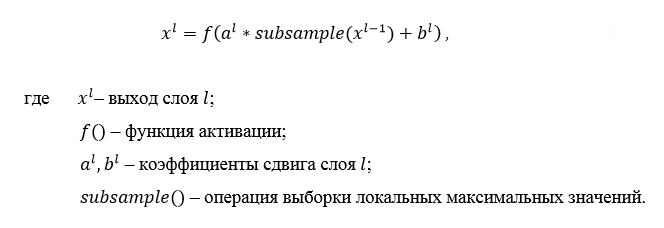
\includegraphics[width=0.8\linewidth]{pool_l}
		\end{minipage}
	\end{center}
\end{figure}

\subsection{Полносвязный слой}

Последний из типов слоев это слой обычного многослойного персептрона. Цель слоя~--- классификация, моделирует сложную нелинейную функцию, оптимизируя которую, улучшается качество распознавания. Вычисление значений нейрона можно описать формулой:
	\begin{center}
		$\mathsf{x}_{\mathsf{j}}^{\mathsf{l}} = f(\sum \limits_{\mathsf{i}} \mathsf{x}_{\mathsf{i}}^{\mathsf{l-1}} * \mathsf{w}_{\mathsf{i,j}}^{\mathsf{l-1}}+\mathsf{b}_{\mathsf{j}}^{\mathsf{l-1}})$,
	\end{center}
	где
	\begin{itemize}
		\item $\mathsf{x}_{j}^{l}$ -- карта признаков $\mathsf{j}$ (выход слоя $\mathsf{l}$), 
		\item $f()$ -- функция активации,
		\item $\mathsf{b}^{\mathsf{l}}$ -- коэффициент сдвига слоя $\mathsf{l}$,
		\item $\mathsf{w}_{\mathsf{i,j}}^{\mathsf{l}}$ -- матрица весовых коэффициентов слоя $\mathsf{l}$.
	\end{itemize}


\subsection{Выходной слой}
Выходной слой связан со всеми нейронами предыдущего слоя. Количество нейронов соответствует количеству распознаваемых классов. Но для уменьшения количества связей и вычислений для бинарного случая можно использовать один нейрон и при использовании в качестве функции активации гиперболический тангенс. 

\section{Выбор функции активации}

Одним из этапов разработки нейронной сети является выбор функции активации нейронов. Вид функции активации во многом определяет функциональные возможности нейронной сети и метод обучения этой сети. Классический алгоритм обратного распространения ошибки хорошо работает на двухслойных и трехслойных нейронных сетях, но при дальнейшем увеличении глубины начинает испытывать проблемы. Одна из причин~— так называемое затухание градиентов. По мере распространения ошибки от выходного слоя к входному на каждом слое происходит домножение текущего результата на производную функции активации. Производная у традиционной сигмоидной функции активации меньше единицы на всей области определения, поэтому после нескольких слоев ошибка станет близкой к нулю. Если же, наоборот, функция активации имеет неограниченную производную (как, например, гиперболический тангенс), то может произойти взрывное увеличение ошибки по мере распространения, что приведет к неустойчивости процедуры обучения.

\subsection{Сигмойда}
Эта функция относится к классу непрерывных функций и принимает на входе произвольное вещественное число, а на выходе дает вещественное число в интервале от 0 до 1. В частности, большие (по модулю) отрицательные числа превращаются в ноль, а большие положительные – в единицу. Исторически сигмоида находила широкое применение, поскольку ее выход хорошо интерпретируется, как уровень активации нейрона: от отсутствия активации (0) до полностью насыщенной активации (1). Сигмоида (sigmoid) выражается формулой: 
\begin{equation*}
\sigma(z) = \frac{1}{1 - e^{-az}}, a \in \mathbb{R}
\end{equation*}
\subsection{Гиперболический тангенс}

Еще одна часто используемая активационная функция — гиперболический тангенс, формула которой:  
\begin{equation*}
\sigma(z) = \frac{e^{az} - e^{-az}}{e^{az} + e^{-az}}.
\end{equation*}

Гиперболический тангенс очень похож на сигмоиду. И действительно, это скорректированная сигмоидная функция. Поэтому такая функция имеет те же характеристики, что и у сигмоиды, рассмотренной ранее. Её природа нелинейна, она хорошо подходит для комбинации слоёв, а диапазон значений функции --- $(-1, 1)$. Поэтому нет смысла беспокоиться, что активационная функция перегрузится от больших значений. Однако стоит отметить, что градиент тангенциальной функции больше, чем у сигмоиды (производная круче). Решение о том, выбрать ли сигмоиду или тангенс, зависит от требований к амплитуде градиента. Также как и сигмоиде, гиперболическому тангенсу свойственная проблема исчезновения градиента.


\subsection{RelU}

Известно, что нейронные сети способны приблизить сколь угодно сложную функцию, если в них достаточно слоев и функция активации является нелинейной. Функции активации вроде сигмоидной или тангенциальной являются нелинейными, но приводят к проблемам с затуханием или увеличением градиентов. Однако можно использовать и гораздо более простой вариант — выпрямленную линейную функцию активации (rectified linear unit, ReLU), которая выражается формулой:  

\begin{equation*}
	\sigma(z) = max(0,z)
\end{equation*}

Преимущества использования ReLU:

\begin{itemize}
	\item ее производная равна либо единице, либо нулю, и поэтому не может произойти разрастания или затухания градиентов, т.к. умножив единицу на дельту ошибки мы получим дельту ошибки, если же мы бы использовали другую функцию, например, гиперболический тангенс, то дельта ошибки могла, либо уменьшиться, либо возрасти, либо остаться такой же, то есть, производная гиперболического тангенса возвращает число с разным знаком и величиной, что можно сильно повлиять на затухание или разрастание градиента. Более того, использование данной функции приводит к прореживанию весов;
	\item вычисление сигмоиды и гиперболического тангенса требует выполнения ресурсоемких операций, таких как возведение в степень, в то время как ReLU может быть реализован с помощью простого порогового преобразования матрицы активаций в нуле;
	\item отсекает ненужные детали в канале при отрицательном выходе.
\end{itemize}

Из недостатков можно отметить, что ReLU не всегда достаточно надежна и в процессе обучения может выходить из строя («умирать»). Например, большой градиент, проходящий через ReLU, может привести к такому обновлению весов, что данный нейрон никогда больше не активируется. Если это произойдет, то, начиная с данного момента, градиент, проходящий через этот нейрон, всегда будет равен нулю. Соответственно, данный нейрон будет необратимо выведен из строя. 

\subsection{Softmax}

Softmax — это обобщение логистической функции для многомерного случая. Функция преобразует вектор $z$ размерности $K$ в вектор $\sigma$ той же размерности, где каждая координата 
$\sigma_{i}$ полученного вектора представлена вещественным числом в интервале [0,1] и сумма координат равна 1. Координаты $\sigma_{i}$ вычисляются следующим образом:

\begin{equation*}
	\sigma(z)_{\mathsf{i}} = \frac{e^{z_{\mathsf{i}}}}{\sum \limits_{k=1}^{K} e^{z_{k}} }
\end{equation*}


\section{Обучение сверточной нейронной сети}

На начальном этапе нейронная сеть является необученной (ненастроенной). В общем смысле под обучением понимают последовательное предъявление образа на вход нейросети, из обучающего набора, затем полученный ответ сравнивается с желаемым выходом, полученная разница между ожидаемым ответом и полученным является результат функции ошибки (дельта ошибки). Затем эту дельту ошибки необходимо распространить на все связанные нейроны сети. 

Таким образом обучение нейронной сети сводится к минимизации функции ошибки, путем корректировки весовых коэффициентов синаптических связей между нейронами. Под функцией ошибки понимается разность между полученным ответом и желаемым.  Затем веса выходного слоя нейронов корректируются в соответствии с ошибкой. Для нейронов выходного слоя известны их фактические и желаемые значения выходов. Поэтому настройка весов связей для таких нейронов является относительно простой. Однако для нейронов предыдущих слоев настройка не столь очевидна. Долгое время не было известно алгоритма распространения ошибки по скрытым слоям.

\subsection{Алгоритм обратного распространения ошибки}

Для обучения описанной нейронной сети был использован алгоритм обратного распространения ошибки (backpropagation). Этот метод обучения многослойной нейронной сети называется обобщенным дельта-правилом.  Данный алгоритм является первым и основным практически применимым для обучения многослойных нейронных сетей. 

Для выходного слоя корректировка весов интуитивна понятна, но для скрытых слоев долгое время не было известно алгоритма. Веса скрытого нейрона должны изменяться прямо пропорционально ошибке тех нейронов, с которыми данный нейрон связан. Вот почему обратное распространение этих ошибок через сеть позволяет корректно настраивать веса связей между всеми слоями. В этом случае величина функции ошибки уменьшается и сеть обучается. 

Основные соотношения метода обратного распространения ошибки получены при следующих обозначениях:
\begin{figure}[h]
	\begin{center}
		\begin{minipage}[h]{1\linewidth}
			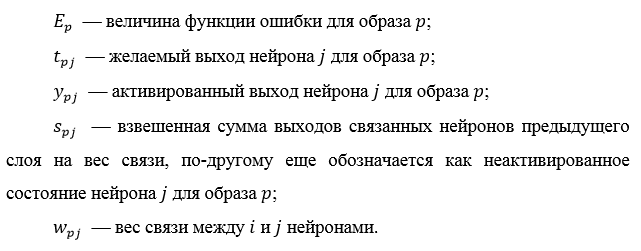
\includegraphics[width=0.7\linewidth]{back_prop_1}
		\end{minipage}
	\end{center}
\end{figure}

Величина ошибки определяется по формуле:
\begin{figure}[h]
	\begin{center}
		\begin{minipage}[h]{1\linewidth}
			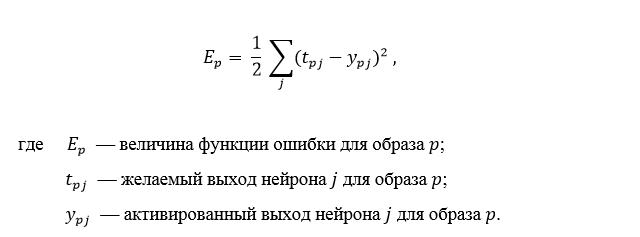
\includegraphics[width=0.7\linewidth]{back_prop_2}
		\end{minipage}
	\end{center}
\end{figure}

Неактивированное состояние каждого нейрона j для образа p записывается в виде взвешенной суммы по формуле:
\begin{figure}[!h]
	\begin{center}
		\begin{minipage}[!h]{1\linewidth}
			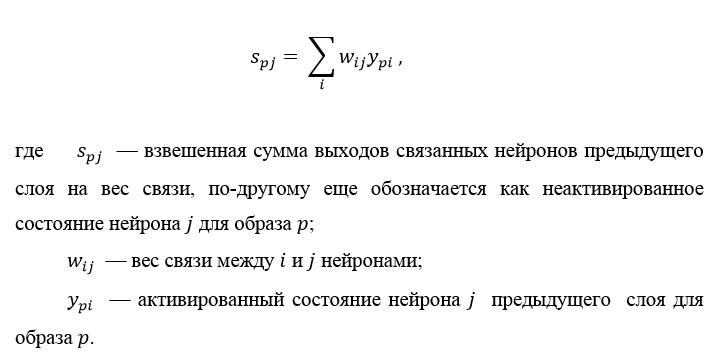
\includegraphics[width=0.7\linewidth]{back_prop_3}
		\end{minipage}
	\end{center}
\end{figure}

Выход каждого нейрона j является значением активационной функции $f_j$, которая переводит нейрон в активированное состояние. В качестве функции активации может использоваться любая непрерывно дифференцируемая монотонная функция. Активированное состояние нейрона вычисляется по формуле:
\begin{figure}[!h]
	\begin{center}
		\begin{minipage}[!h]{1\linewidth}
			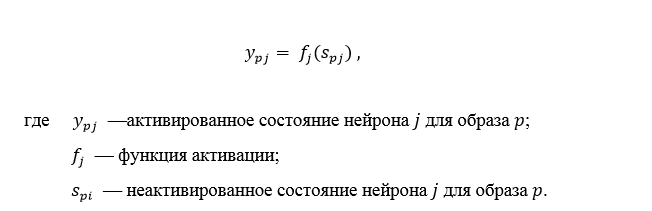
\includegraphics[width=0.7\linewidth]{back_prop_4}
		\end{minipage}
	\end{center}
\end{figure}

В качестве метода минимизации ошибки используется метод градиентного спуска, суть этого метода сводится к поиску минимума (или максимума) функции за счет движения вдоль вектора градиента. Для поиска минимума движение должно быть осуществляться в направлении антиградиента. Градиент функции потери представляет из себя вектор частных производных, вычисляющийся по формуле:
\begin{figure}[!h]
	\begin{center}
		\begin{minipage}[!h]{1\linewidth}
			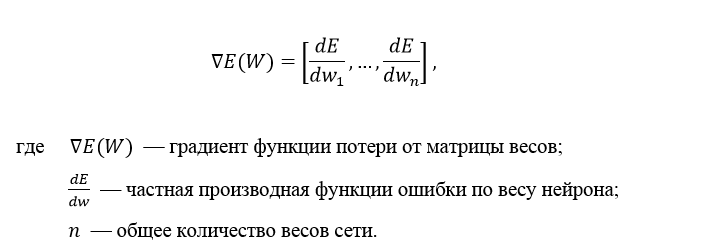
\includegraphics[width=0.7\linewidth]{back_prop_5}
		\end{minipage}
	\end{center}
\end{figure}

Производную функции ошибки по конкретному образу можно записать по правилу цепочки:
\begin{figure}[!h]
	\begin{center}
		\begin{minipage}[!h]{1\linewidth}
			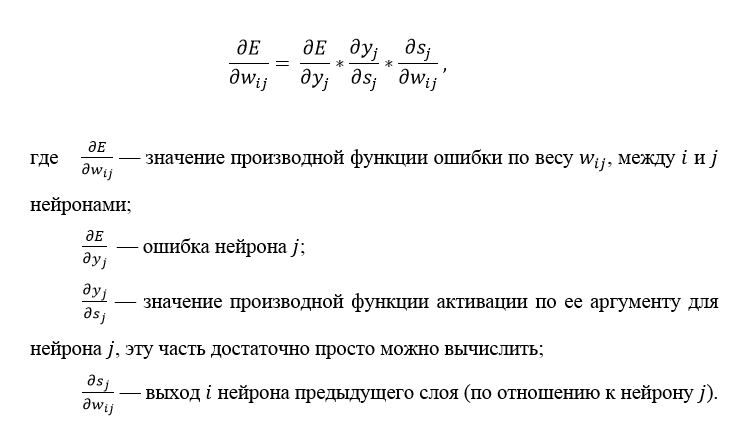
\includegraphics[width=0.7\linewidth]{back_prop_6}
		\end{minipage}
	\end{center}
\end{figure}

Ошибка нейрона $\frac{\partial E}{\partial y_j}$  обычно записывается в виде символа $\delta$ (дельта). Для выходного слоя ошибка определена в явном виде, если взять производную от ошибки, то получим t минус y, то есть разницу между желаемым и полученным выходом. Но как рассчитать ошибку для скрытых слоев? Для решения этой задачи, как раз и был придуман алгоритм обратного распространения ошибки. Суть его заключается в последовательном вычислении ошибок скрытых слоев с помощью значений ошибки выходного слоя, т.е. значения ошибки распространяются по сети в обратном направлении от выхода к входу. 
Ошибка $\delta$ для скрытого слоя рассчитывается по формуле:
\begin{figure}[!h]
	\begin{center}
		\begin{minipage}[!h]{1\linewidth}
			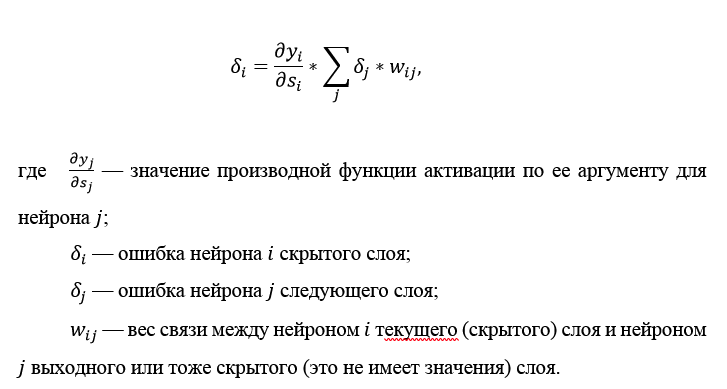
\includegraphics[width=0.7\linewidth]{back_prop_7}
		\end{minipage}
	\end{center}
\end{figure}

Алгоритм распространения ошибки сводится к следующим этапам:
\begin{itemize}
	\item прямое распространение сигнала по сети, вычисления состояния нейронов;
	\item вычисление значения ошибки $\delta$ для выходного слоя;
	\item обратное распространение: последовательно от конца к началу для всех скрытых слоев вычисляем $\delta$;
	\item обновление весов сети на вычисленную ранее $\delta$ ошибки.
\end{itemize}

До этого момента были рассмотрены случаи распространения ошибки по слоям персептрона, то есть по выходному и скрытому, но помимо них, в сверточной нейросети имеются объединяющий и сверточный. 

\subsection{Расчет ошибки на подвыборочном слое}

Расчет ошибки на объединяющем слое представляется в нескольких вариантах. Первый случай, когда объединяющий слой находится перед полносвязным, тогда он имеет нейроны и связи такого же типа, как в полносвязном слое, соответственно вычисление $\delta$ ошибки ничем не отличается от вычисления $\delta$ скрытого слоя. Второй случай, когда подвыборочный слой находится перед сверточным, вычисление $\delta$ происходит путем обратной свертки. Для понимания обратно свертки, необходимо сперва понять обычную свертку и то, что скользящее окно по карте признаков (во время прямого распространения сигнала) можно интерпретировать, как обычный скрытый слой со связями между нейронами, но главное отличие — это то, что эти связи разделяемы, то есть одна связь с конкретным значением веса может быть у нескольких пар нейронов, а не только одной.

 Интерпретация операции свертки в привычном многослойном виде:
 \begin{figure}[!h]
 	\begin{center}
 		\begin{minipage}[!h]{1\linewidth}
 			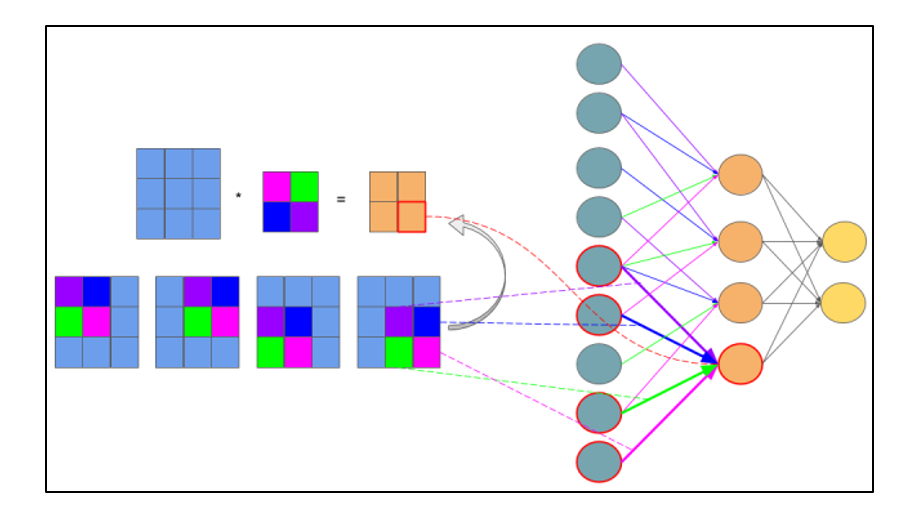
\includegraphics[width=0.75\linewidth]{pic1}
 		\end{minipage}
 	\end{center}
 \end{figure}
 
 Теперь, когда операция свертки представлена в привычном многослойном виде, можно интуитивно понять, что вычисление дельт происходит таким же образом, как и в скрытом слое полносвязной сети. Соответственно имея вычисленные ранее дельты сверточного слоя можно вычислить дельты объединяющего:
  \begin{figure}[!h]
 	\begin{center}
 		\begin{minipage}[!h]{1\linewidth}
 			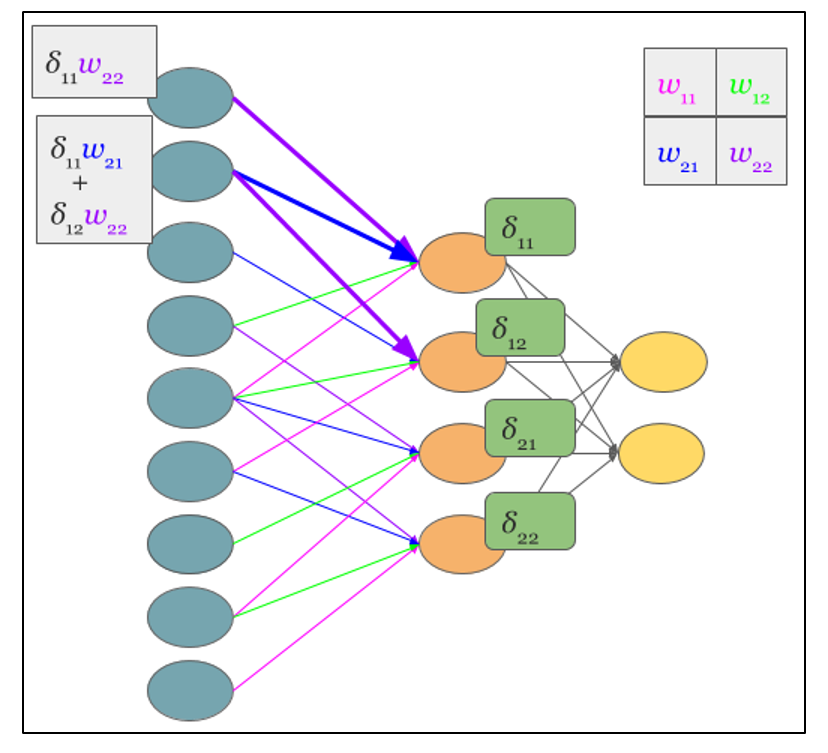
\includegraphics[width=0.75\linewidth]{pic2}
 		\end{minipage}
 	\end{center}
 \end{figure}
 
 Обратная свертка –-- это тот же самый способ вычисления дельт, только немного хитрым способом, заключающийся в повороте ядра на 180 градусов и скользящем процессе сканирования сверточной карты дельт с измененными краевыми эффектами. Простыми словами, нам необходимо взять ядро сверточной карты (следующего за объединяющим слоем) повернуть его на 180 градусов и сделать обычную свертку по вычисленным ранее дельтам сверточной карты, но так чтобы окно сканирования выходило за пределы карты. Результат операции обратной свертки:
   \begin{figure}[!h]
 	\begin{center}
 		\begin{minipage}[!h]{1\linewidth}
 			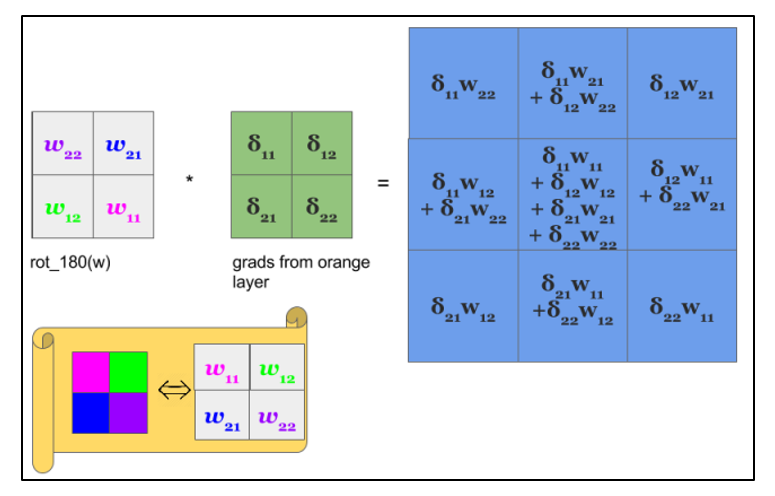
\includegraphics[width=0.75\linewidth]{pic3}
 		\end{minipage}
 	\end{center}
 \end{figure}

 Цикл прохода обратной свертки:
   \begin{figure}[!h]
	\begin{center}
		\begin{minipage}[!h]{1\linewidth}
			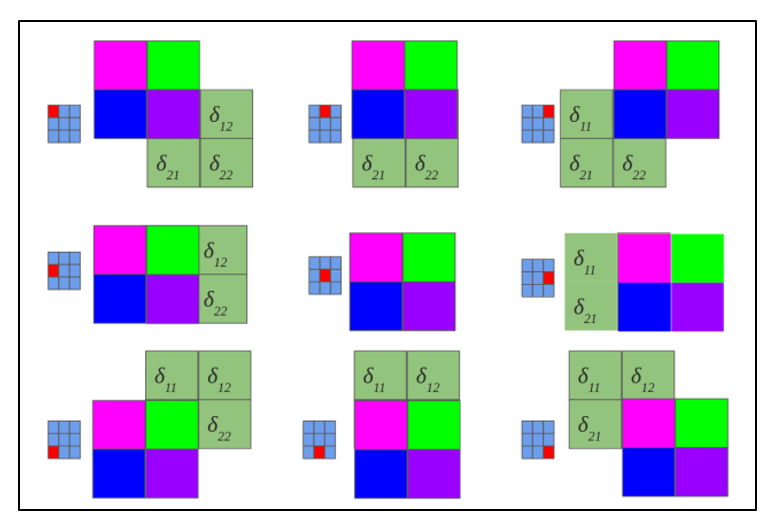
\includegraphics[width=0.75\linewidth]{pic4}
		\end{minipage}
	\end{center}
\end{figure}

\subsection{Расчет ошибки на сверточном слое}

Обычно впередиидущий слой после сверточного это объединяющий, соответственно наша задача вычислить дельты текущего слоя (сверточного) за счет знаний о дельтах объединяющего слоя. На самом деле дельта ошибка не вычисляется, а копируется. При прямом распространении сигнала нейроны объединяющего слоя формировались за счет неперекрывающегося окна сканирования по сверточному слою, в процессе которого выбирались нейроны с максимальным значением, при обратном распространении, мы возвращаем дельту ошибки тому ранее выбранному максимальному нейрону, остальные же получают нулевую дельту ошибки.

\subsection{Заключение}

Представив операцию свертки в привычном многослойном виде, можно интуитивно понять, что вычисление дельт происходит таким же образом, как и в скрытом слое полносвязной сети. 

\end{document}